\newcommand{\Morph}{u}

\chapter{Computational aspects}

\section{Systems of chemical reactions}
Reaction-diffusion equations are an idealized and abstract representation of reality. They comprise two phenomena, chemical reactions and diffusion. Mathematically, this is represented as a system of partial differential equations (PDEs). Whose numerical solution requires discretization of time and space. Computation of chemical reactions at a point in space, only depend on the elapsed time and previous concentration. However, the computation of diffusion is more complicated, and depends additionally on the concentrations in the areas adjacent to the point of interest.

\section{Isotropic Diffusion}
Diffusion is an integral part of natural patterning models. It is the process in which particles of a substance move from high to low concentrations. This change in concentration over space is referred to as a gradient. Diffusion driven by gradients was first explored by Adolf Fick \citep{fick1995liquid}. The diffusion of a chemical concentration $\Morph$ was formalized in 1855 by Fick's second law:
\begin{equation}
\label{eq:ficks2ndlaw0}
	\frac{\partial \Morph}{\partial t} = \Div (D \nabla \Morph).
\end{equation}
	
$\Div$ is the divergence operator, $\nabla$ is the gradient operator, and $u$ is a scalar field. Given Eqn \ref{eq:ficks2ndlaw0}, we see that the diffusion rate depends on the gradient of the concentration. At a given location, the divergence of the gradient measures the difference between the concentration at that point and the average of the neighbouring concentrations. This divergence measurement is proportional to the change in concentration due to diffusion. But, particle size and domain porosity also affect the diffusion rate. This is represented as the diffusivity coefficient $D$. If diffusivity is the same regardless of direction, this diffusion is said to be isotropic and we can simplify Eqn \ref{eq:ficks2ndlaw0} as:
\begin{equation}
\label{eq:ficks2ndlaw1}
	\frac{\partial \Morph}{\partial t} = D \Lap \Morph.
\end{equation}
	
$\Lap$ is the divergence of the gradient and is called the Laplacian. Formally, it is the sum of the second spatial derivative in each basis direction $x_i$.

\begin{equation}
\label{eq:laplacian}
	\Lap = \sum_{i=0}^{n} \frac{\partial^2}{\partial x_i^2}.
\end{equation}
	
\section{Anisotropic diffusion}
In many biological scenarios, particles do not diffuse at an equal rate in all directions. In that case, the diffusion is called anisotropic and the diffusivity coefficient changes based on the direction considered. For anisotropic diffusion, a single scalar $D$ no longer suffices. We can represent anisotropy by a tensor $\Lambda$. In the two dimensional case, the tensor has the form:
\[\Lambda =
\begin{bmatrix}
    \lambda_1 & 0 \\
    0 & \lambda_2 
\end{bmatrix}\]
Each $\lambda_i$ represents the diffusivity in a basis of our space. Thus, $\Lambda$ is axis-aligned. Arbitrary orientations can be represented with a rotation matrix $R$, allowing us to represent general anisotropic diffusion:
\[D = R^T \Lambda R.\]
Now we can use $D$ to transform our gradient and thereby our diffusion rate:
\begin{equation}
\label{eq:anisoLap}
	\frac{\partial \Morph}{\partial t} = \Div (D \nabla \Morph).
\end{equation}
\section{Discrete diffusion operators}
To simulate reaction-diffusion, the domain on which it is simulated must be discretized, which in turn means that we must use a discrete version of the Laplacian.

\subsection{Diffusion on grids}
Grids of square cells are a common representation of domains. Each cell in the grid has an area associated with concentrations of morphogens. Computationally concentrations are represented by a scalar value assigned to each cell. This has many benefits as grids are easy to represent and the required differential operators are simple to implement.

\subsubsection*{Diffusion in 1D} 
Computing diffusion on a 1D grid of cells can be accomplished by representing the Laplacian through finite differencing operations. Because the Laplacian involves second order derivatives, we can approximate it by computing the difference of two first order differences as shown below for a grid cell centred at $\Morph_i$, where $i$ is the $i^{th}$ cell:
\begin{equation}
\begin{aligned} \label{eq:firstOrderDifference}
	T_0 &= \frac{(\Morph_{i} - \Morph_{i-1})}{h},\\
	T_1 &= \frac{(\Morph_{i+1} - \Morph_i)}{h}.
\end{aligned}
\end{equation}
Here $\Morph_{i-1}, \Morph_i, \Morph_{i+1}$ are morphogen concentrations at their respective grid cells, $T_0$ and $T_1$ are the first order differences, and $h$ is the distance between the centres of adjacent cells. The discrete Laplacian is then:
\begin{equation} 
\label{eq:secondOrderDifference}
	\Lap \Morph_i = \frac{T_1 - T_0}{h} = \frac{\Morph_{i-1} - 2\Morph_i + \Morph_{i+1}}{h^2}.
\end{equation}
This differencing can be represented as a convolution mask during computation, as shown below:
\begin{figure}[!ht]
\centering
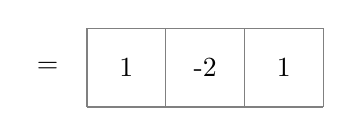
\begin{tikzpicture}
\draw[step=1.0cm,color=gray] (0,0) grid (3,1);
\node at (-0.5,+0.5) {$\Lap =$};
\node at (+0.5,+0.5) {1}; %\node at (+0.5, -0.25) {$f_{i-1}$};
\node at (+1.5,+0.5) {-2}; %\node at (+1.5, -0.25) {$f_i$};
\node at (+2.5,+0.5) {1}; %\node at (+2.5, -0.25) {$f_{i+1}$};
\end{tikzpicture}
\end{figure}	
	%\[\frac{\partial f_i}{\partial t} = \frac{\Lap*f}{h^2} \]
\subsubsection*{Diffusion in 2D}
In this case we have two directions to consider. Recall that the Laplacian is the sum of the second derivatives in each principle direction. This allows us to use the summation of the 1D case in both $x$ and $y$ directions which, for a cell $\Morph_{i,j}$, yields:
	\[\Lap \Morph_{i,j} = \frac{\Morph_{i,j−1} + \Morph_{i,j+1} + \Morph_{i−1,j} + \Morph_{i+1,j} − 4\Morph_{i,j}}{h^2} .\]
Again, the Laplacian operator can be represented as a convolution mask:

\begin{figure}[H]
\centering
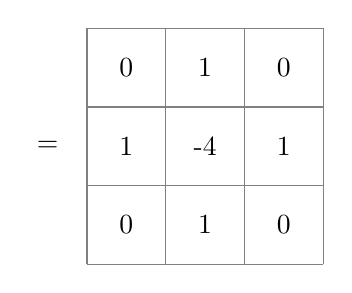
\begin{tikzpicture}
\draw[step=1.0cm,color=gray] (0,0) grid (3,3);
\node at (-0.5,+1.5) {$\Lap =$};
\node at (+0.5,+2.5) {0};
\node at (+1.5,+2.5) {1};
\node at (+2.5,+2.5) {0};
\node at (+0.5,+1.5) {1};
\node at (+1.5,+1.5) {-4};
\node at (+2.5,+1.5) {1};
\node at (+0.5,+0.5) {0};
\node at (+1.5,+0.5) {1};
\node at (+2.5,+0.5) {0};
\end{tikzpicture}
\end{figure}

\subsection{Diffusion on arbitrary triangular meshes}
We represent morphogens on a triangular mesh by assigning them to vertices. But, as with grid based domains, each morphogen concentration is actually associated with an area. The area partitioning on a mesh is the dual cell. This area depends on the mesh triangulation, and can change per vertex. To allow for easy neighbour identification and area calculation, I represent the triangular mesh as a half-edge data structure \citep{Mantyla1988}. 

To build this data structure, each edge in the mesh is replaced by two half-edges. A single half-edge has a pointer to the next half-edge in the same face, as shown in Fig \ref{fig:halfEdgeMesh}. Also, it has a pointer to the vertex that it originates from and a pointer to the complementing half-edge. Each vertex stores a scalar representing the area of the dual cell. For our computation, this area is the sum of one third of each adjacent face's area. %Alternate area partitions are given in \citep{Meyer2003}.

\begin{figure}[H]
	\centering
	\incfig{halfEdgeMesh}
	\caption{Two triangles and their half-edge representation denoted by black arrows.}
	\label{fig:halfEdgeMesh}
\end{figure}

\subsubsection*{Isotropic diffusion on meshes}
To compute diffusion on an arbitrary triangular mesh, we need a discrete Laplacian. This can be generalized as:
\[
(\Lap{} \Morph)_i = \frac{1}{A} \sum_{i \sim j} w_{ij}(\Morph_i - \Morph_j).
\]
This states that the Laplacian at vertex $i$ of the scalar field $\Morph$, is the sum of the weighted differences between the concentration at $i$, $\Morph_i$, and each neighbouring concentrations $\Morph_j$. The weight is $w_{ij}$, each edge is denoted $i \sim j$, and the area associated with $i$ is $A$. We divide the sum by $A$ to get the concentration at the vertex, instead of the area. The choice of weight determines the behaviour of the Laplacian. It has been shown that no discretization maintains all the properties of the continuous Laplacian \citep{Wardetzky2007}. The most common weighting used is the cotangent Laplacian:

\begin{equation}
	(\Lap{} \Morph)_i = \frac{1}{2A} \sum_{i \sim j} (cot(\alpha) + cot(\beta)) (\Morph_i - \Morph_j).
	\label{eq:cotanLaplacian}
\end{equation}

The cotangent weights are computed from the angles opposite the current edge. This weight can be derived from the ratio of the edge length of the dual cell and the current edge's length. The current edge length is an inverse coefficient of the morphogen gradient between $i$ and $j$. The length of the dual cell edge represents how much of an interface between the areas exists. When this is larger, diffusion increases. These are represented in Fig \ref{fig:dualMesh}. To find the cotangent Laplacian for the entire mesh we evaluate Eqn \ref{eq:cotanLaplacian} at each vertex. A rigorous derivation is given in \citep{Crane2013DGP}. The drawback of this Laplacian compared to the continuous version is that the cotangent weights can be negative. This occurs when angles are greater than $90^\circ$. Consequently, care must be taken when meshing your domain.

\begin{figure}[H]
	\centering
	\incfig{dualMesh}
	\caption{A vertex $i$ and its dual area $A$. The weighting for the cotangent Laplacian between vertex $i$ and $j$ is dependant on the length of the red and black edges.}
	\label{fig:dualMesh}
\end{figure}


\subsubsection*{Anisotropic diffusion on meshes}
To simulate anisotropic diffusion on a triangular mesh, each vertex is assigned the two diffusivity scalars and a diffusion direction vector. For each face adjacent to our vertex, $\Lambda$ is oriented with $R$. To construct $R$, the face normal and a face direction (an angle-weighted average of the vertex directions projected onto the face) are used. $D$ is now used to transform the morphogen gradient on each face. From this we can build a matrix, $L$, representing discrete anisotropic Laplacian operator:

\[ 
   L_{ij} =
   \begin{cases} 
      -\frac{1}{2A}\sum\limits_{t} \frac{D^\perp e_i}{\norm{e_i}} \cdot \frac{e_i}{\norm{e_i}}(cot(\alpha)+cot(\theta))  & i = j \\
      \frac{1}{2A}(\Gamma \frac{cos(\gamma)}{sin(\alpha)} + \Xi\frac{cos(\xi)}{sin(\beta)})   & i \sim j \\
      0 & otherwise
   \end{cases}
\]
This matrix is used to compute diffusion when given a vector of morphogen concentrations, $u$, by:
\[
	Lu = \Lap u.
\]
This Laplacian is more complicated than before and a complete derivation is given in \citep{AndreuxMathieu2014}. Again, $i$ and $j$ are vertices. $e_i$ and $e_j$ are edges, as shown in Fig \ref{fig:meshLaplacian}. $D^\perp = Q^T D Q$ where $Q$ is a $90^\circ$ rotation matrix about the face normal. This rotation will be used get a vector in the direction of a face gradient. The face gradient vector is then transformed by our diffusion tensor, $D$. The amount that this vector is transformed determines the Laplacian weighting. 

$\Gamma = \frac{\norm{D^\perp e_j}}{\norm{e_j}}$ and $\gamma$ is the angle between $e_i$ and $D^\perp e_j$. Which ensures that if the $D^{\perp} = I$ then $\gamma = \alpha$ and we have regular isotropic diffusion. $\Xi$ and $\xi$ are the same quantities measured on the adjacent triangle with that triangle's $D$. 

\begin{figure}[H]
	\centering
	\incfig{meshLaplacian}
	\caption{Two triangles with their angles and edges associated with the anisotropic cotangent Laplacian.}
	\label{fig:meshLaplacian}
\end{figure}

\section{Boundary Conditions}
When computing the discrete Laplacian, a boundary edge will have only one flanking angle. The other angle is assumed to be 0. This is equivalent to \Quotes{no-flux} boundary conditions or Neumann set to 0. To specify Dirichlet boundary conditions, the time step at boundary vertices can be set 0. This freezes the concentrations found along the boundary. If the concentrations are 0, then the boundary acts as a morphogen sink. Higher values can also be used to represent morphogen sources.

\section{Systems with dynamic structure}
In nature, domains often grow over time which has an appreciable effect on pattern formation. One of them is a diluting effect on chemical concentrations that make up a pattern\footnote{Dilution is often ignored in simulations.}. When simulating directly on triangular meshes, growth changes the range of representable patterns. This is because morphogens are stored and visualized at the vertices, thus the triangle's area represents a minimum size of pattern detail that can be represented. To address this we must use subdivision algorithms to split large triangles into a few smaller ones. Subdividing every face in the mesh can lead to small triangles to be subdivided unnecessarily and the total amount of triangles to grow very quickly. This is a problem because performance of the simulation is determined by the number of vertices that have to be considered. 

Adaptive subdivision is a technique used to only subdivide triangles with an area larger than a given threshold. This approach allows all triangles to maintain a similar area and limits unnecessary creation of triangles. The choice of adaptive subdivision algorithm used determines the shape of the generated triangles. An equilateral triangle is the desired shape for the mesh triangles and large angle deviations from $60^{\circ}$ can pose a problem for the simulation. The number and magnitude of deviations in a mesh give an informal notion of mesh quality. This affects the stability and appearance of the simulation. Depending on the angle, the cotangent weights can be negative or widely varying due to the behaviour of cotan around 0 and 180 degrees. Negative cotangent weights cause diffusion to incorrectly move morphogens from low to high concentrations \citep{Wardetzky2007}. 

\begin{figure}[H]
	\centering
	\incfig{recursiveSubdiv}
	\caption{Subdividing a face, shown in red, using longest-edge bisection.}
	\label{fig:recursiveSubdiv}
\end{figure}

To obtain optimal incremental triangulation that tends to produce good quality triangles, we use longest-edge bisection \citep{RIVARA1998}. In this method, faces are only ever subdivided with respect to their longest edge. A face is subdivided when its area grows past a threshold. If there is an adjacent face to the subdivided edge, we now must subdivide that face to keep the mesh triangular. We recursively apply longest-edge bisection to the adjacent face until its longest edge corresponds to the first longest edge. This recursive subdivision may produce more non triangle faces that will need to be processed in the same way. This process is shown in Fig \ref{fig:recursiveSubdiv}. Upon subdivision of a face, the longest edge is bisected with a new vertex. The concentration assigned to the new vertex is the average of the neighbouring concentration values that shared the edge.

\begin{algorithm}[!ht]
  \KwIn{Triangle t0}
  \KwResult{Triangle is subdivided along its longest edge. Adjacent triangles are recursively subdivided to share edges.}
  \SetKwFunction{subdivide}{subdivide}
  \SetKwProg{myalg}{}{}{}
  \myalg{\subdivide{Triangle t0}}
  {
   Edge \textit{e0 = getLongestEdge(t0)}\\
   bool \textit{subdividing = hasAdjacentFace(e0)}\\
   \textit{subdivideFace(t0, e0)}\\
   \While{subdividing}
   {
    \eIf{hasAdjacentFace(e0)}
    {
      Triangle \textit{t1 = getAdjacentFace(e0)}\\
      Edge \textit{e1 = getLongestEdge(t1)}\\
      \eIf{e1 == getPairEdge(e0)}
      {
       \textit{subdivideFace(t1, e1)}\\
       \textit{subdividing = false}\\
      }{
        \textit{subdivide(t1)}\\   
      }
    }{
     \textit{subdividing = false}\\
    }
   }
  }
  \textbf{end}
  \caption{An algorithm to recursively subdivide a triangle and its neighbours based on \citep{RIVARA1998}.}
  \label{alg:subdivisionAlgorithm}
\end{algorithm}

\section{Numerical methods}
The simulation is advanced by taking small steps through time from a given initial condition. I use the forward Euler method \citep{solomon2015numerical} to perform this integration. A simplified one morphogen reaction-diffusion formula integrated with forward Euler is:

\[
	x_{i+1} = x_{i} + (\Lap{}x_i + F(x_i))\Delta t. \\
\] 

Here $x_i$ is a vector of scalars representing morphogen concentrations at step $i$ and $\Delta t$ is the time-step. $\Lap{}$ is the discrete Laplacian used to compute diffusion and $F(x_i)$ encapsulates the reactions of the system. This method suffers from inaccuracy at larger time-steps because we are assuming $\Lap{}x_i + F(x_i)$ is constant for the whole time-step. This inaccuracy can cause instability in stiff equations by accruing error with each simulation step. Semi-implicit integration schemes exist \citep{Nie2006} allowing for larger time-steps, but in practice, it is possible to use small enough time-steps to minimize inaccuracy and avoid instability. 